\documentclass{article}
\usepackage{amsmath}
\usepackage{graphicx}
\usepackage{float}

\begin{document}

Mijn ideetje is als volgt: statistiek verzamelen over de correlatie van letterfrequenties $f_i$ met de eerste eigenvector van $A$, $v_1$. Als volgt:

\begin{enumerate}
\item Genereer de adjacency-matrix $A\:(N\times N)$ van de (verlengde) ciphercode en bereken zijn eerste eigenvector $v_1$.
\item Genereer de substitutiematrix $S'$ aan de hand van de bekende plaintext, gedefinieerd als volgt: 
$$
    S'_{ij} = \text{aantal keer dat cipherpair $i$ het karakter $j$ codeert}
$$
$S'$ is dus $N\times 26$, en bevat informatie over welke letters worden gecodeerd door ieder paar en hoe vaak.
\item Bereken de genormaliseerde substitutiematrix $S$, verkregen door de som over iedere rij op 1 te normaliseren:
$$
    S_{ij} = \frac{S'_{ij}}{\sum_j S'_{ij}}
$$
\item Bepaal het product $F = Sf$, waar $f$ de $26\times 1$ frequentie vector is. Ieder element van $F\:(N\times 1)$ is nu een lineaire combinatie van frequenties, gewogen door de mate waarin ze voorkwamen in de code. In veel gevallen zal er een 1 op 1 mapping tussen het cipherpaar en de plaintext zijn, in welk geval $F_i = f_i$.

\item Plot $F$ tegen $v_1$:\\
\begin{minipage}{\textwidth}
    \begin{center}
        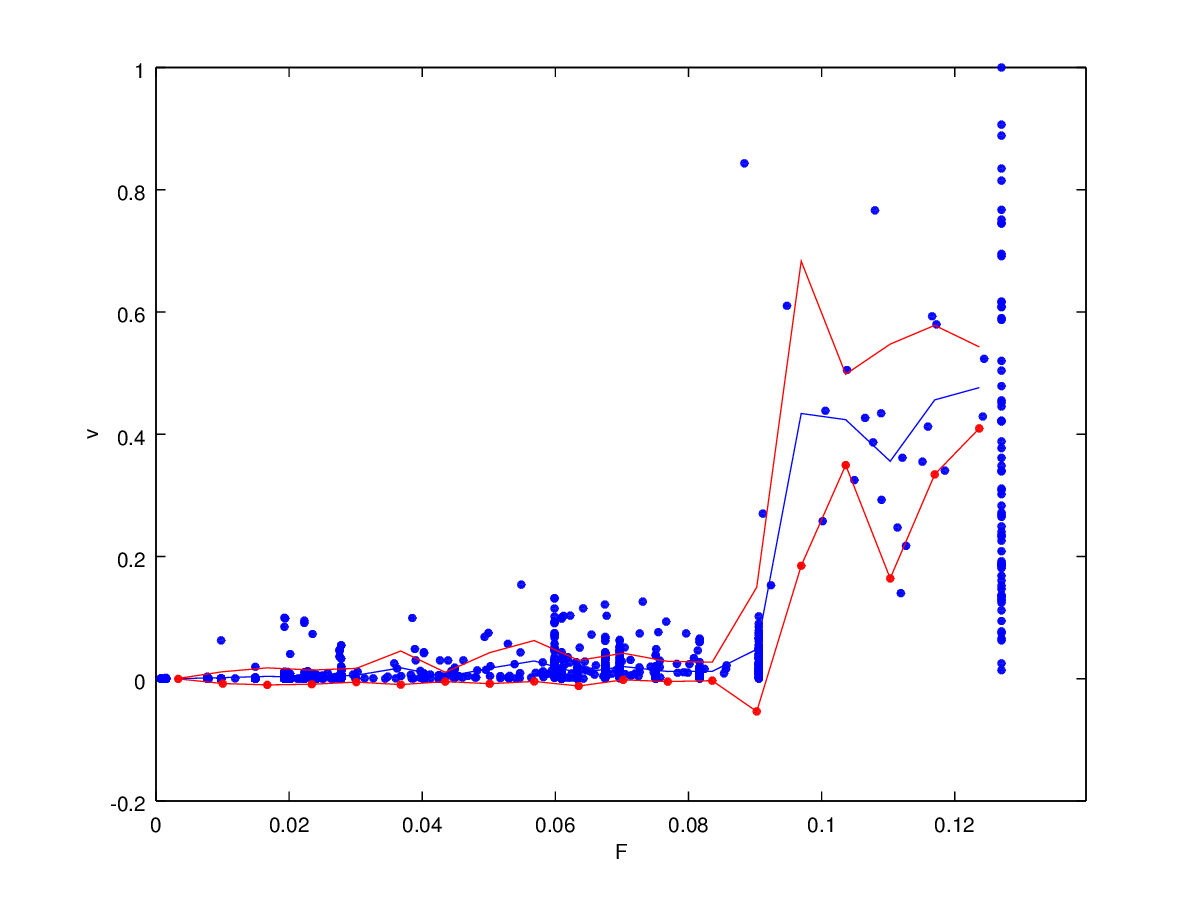
\includegraphics[width=\textwidth]{non_random_correlation}
    \end{center}
\end{minipage}
Belangrijke letters (hoge $F$) lijken gecorelleerd aan een hoge centrality. De blauwe lijn geeft de trend weer en de rode lijn de fout in die trend.

\item Voor een stuk random uniform verdeelde tekst ($f_i = 1/26$) gebeurt het volgende:\\
\begin{minipage}{\textwidth}
    \begin{center}
        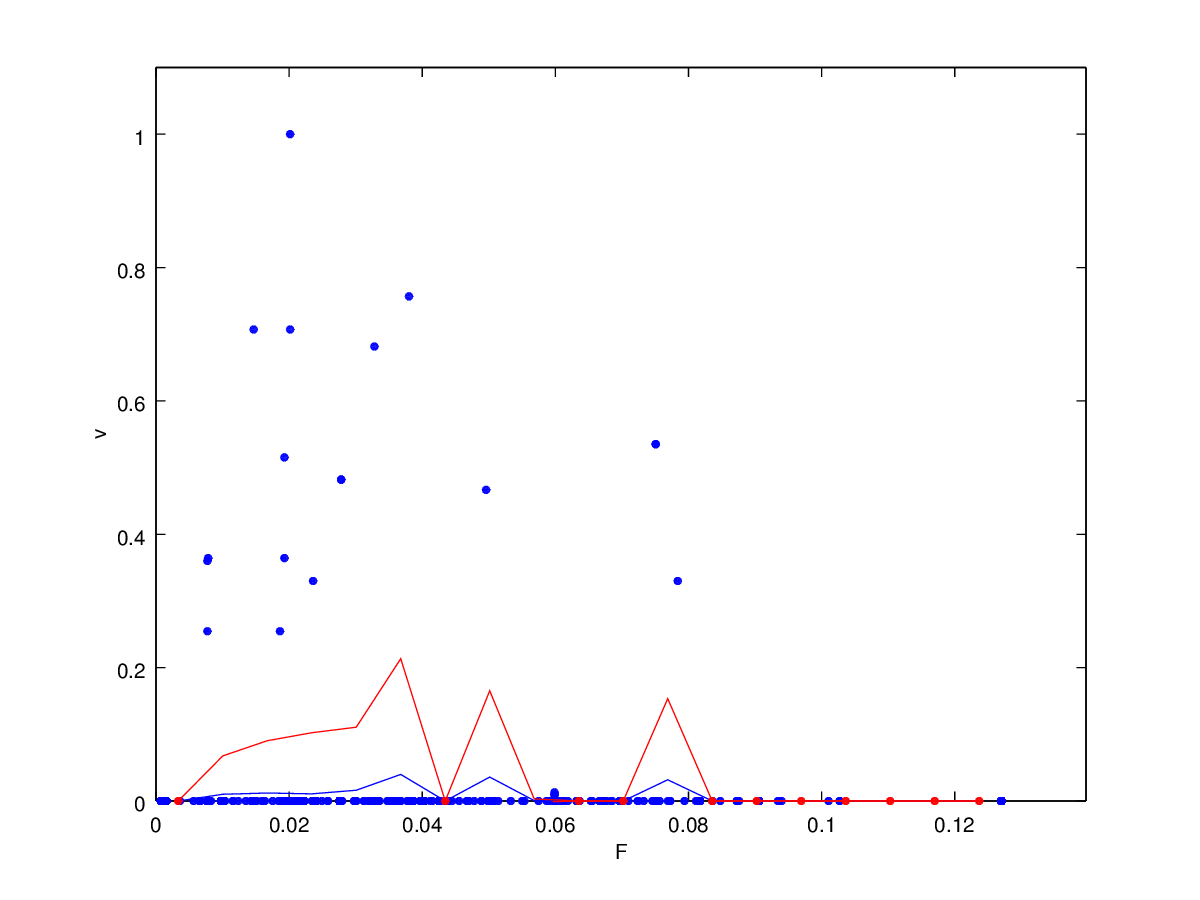
\includegraphics[width=\textwidth]{random_correlation}
    \end{center}
\end{minipage}
De (willekeurige) outliers hebben nauwelijks invloed op het gemiddelde (blauwe lijn).
\end{enumerate}

Wat zeg je ervan? xx Joren

\end{document}
